\begin{figure}[h!]
    \centering
    \caption{Changes in Chicago-Naperville-Elgin CBSA due to a counterfactual raise 
    	     of the federal MW to \$9 in January 2020}
    \label{fig:map_chicago_cf_changes}
	\begin{subfigure}{.67\textwidth}
		\caption{Counterfactual changes in log rents}
		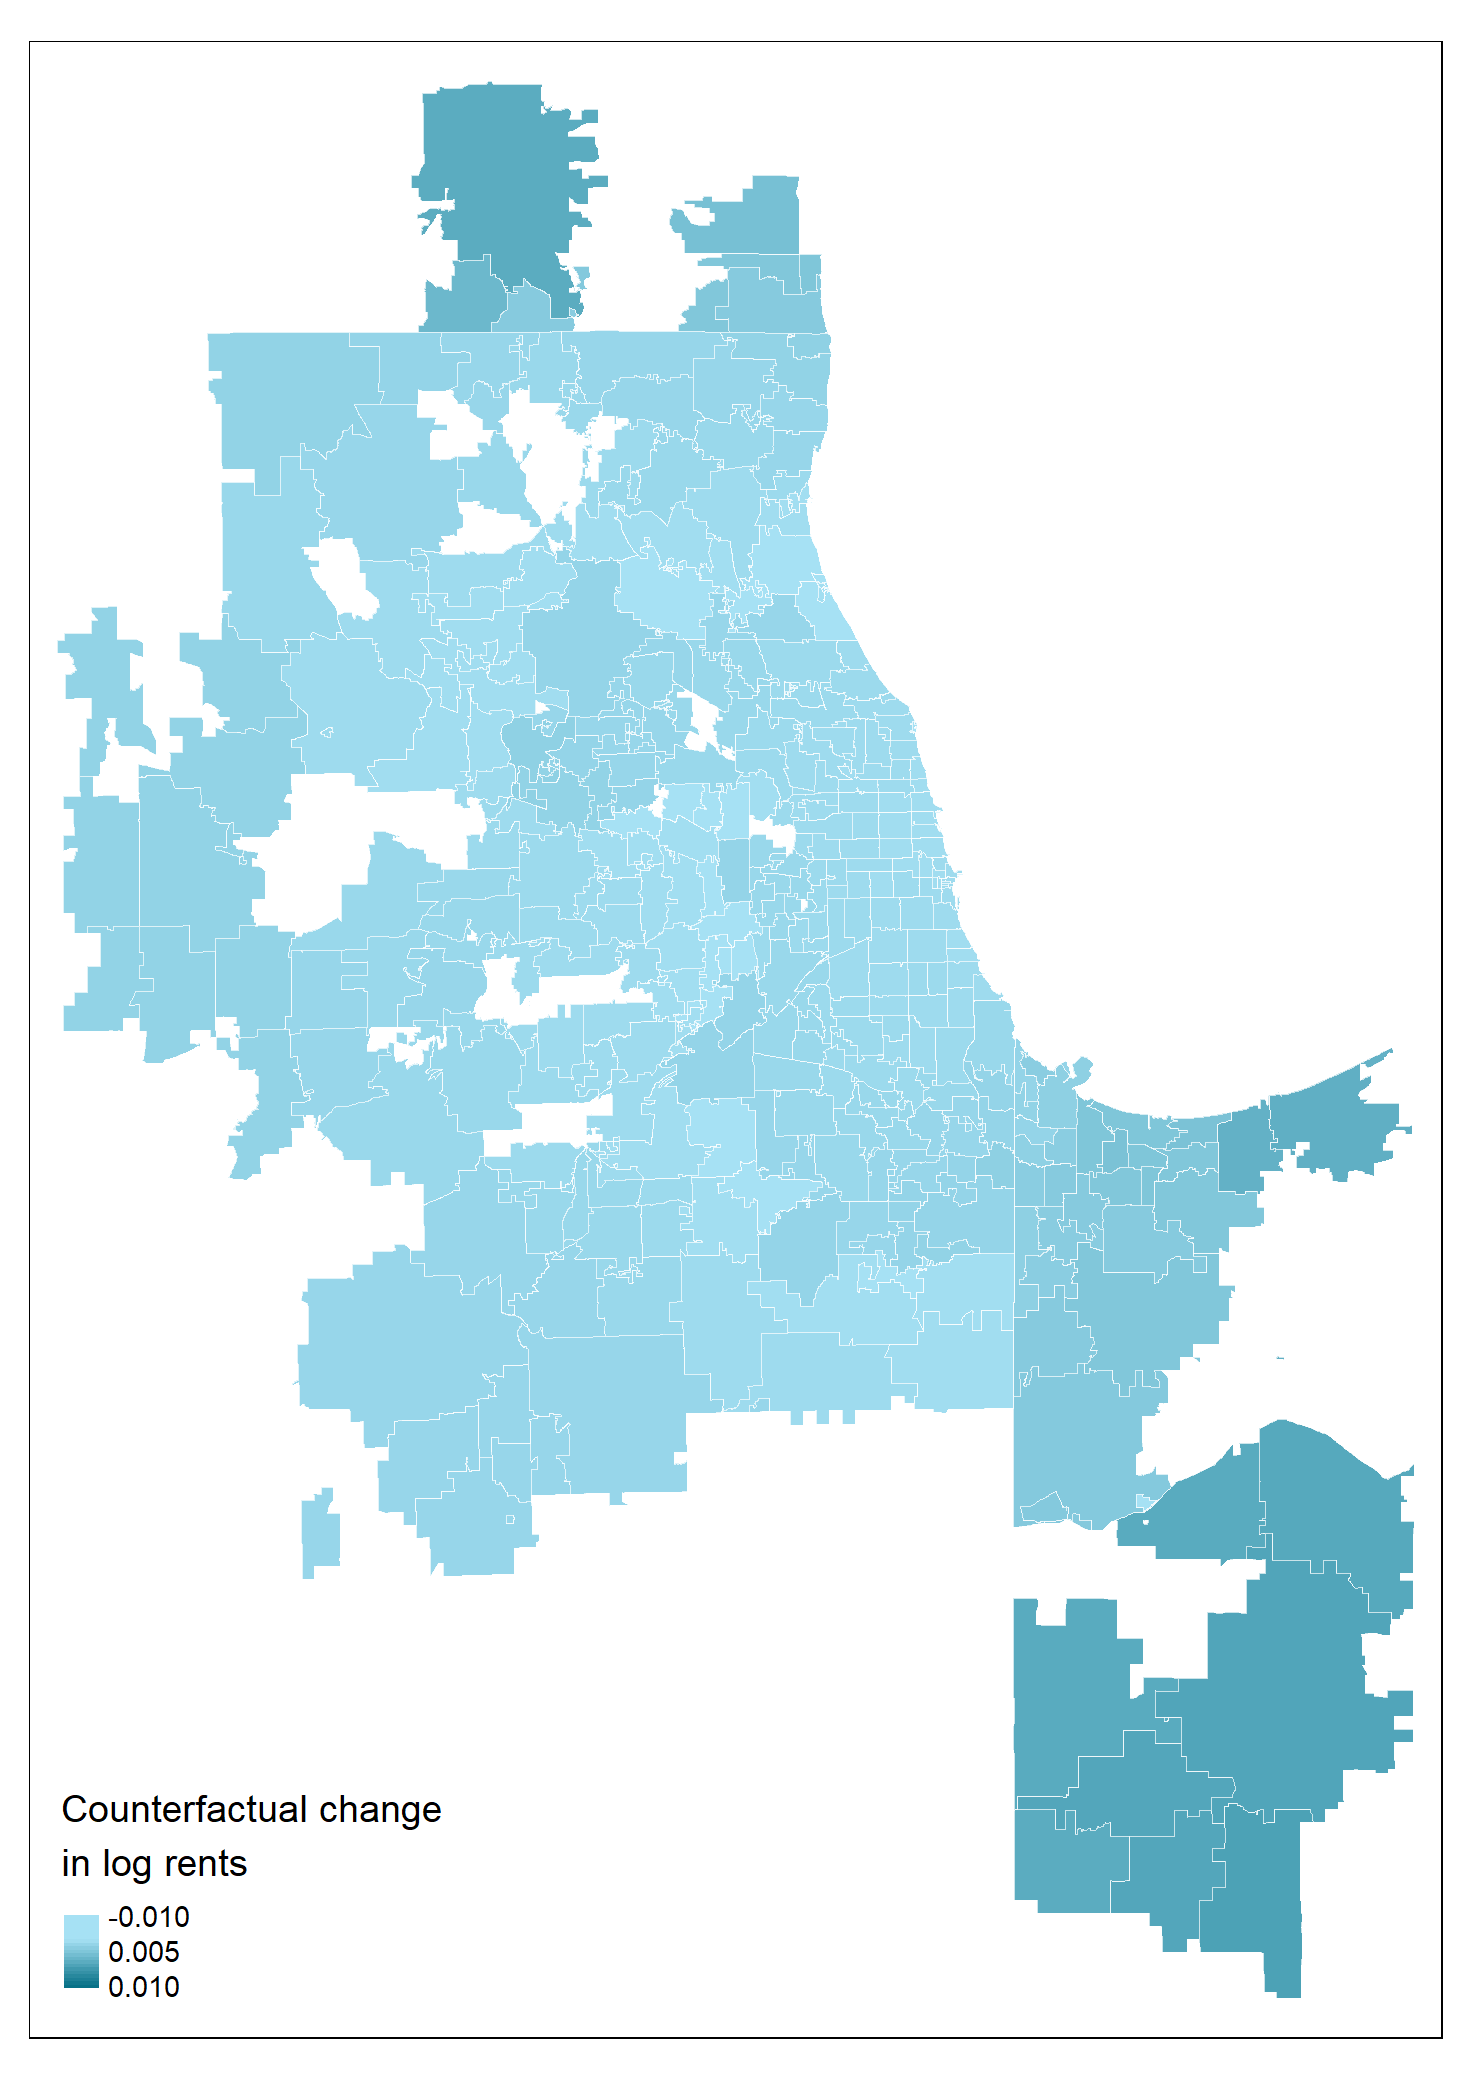
\includegraphics[width = 0.7\textwidth]
		{counterfactuals/output/chicago_d_ln_rents.png}
	\end{subfigure} \\
    \begin{subfigure}{.49\textwidth}
        \caption{Counterfactual changes in residence MW}
        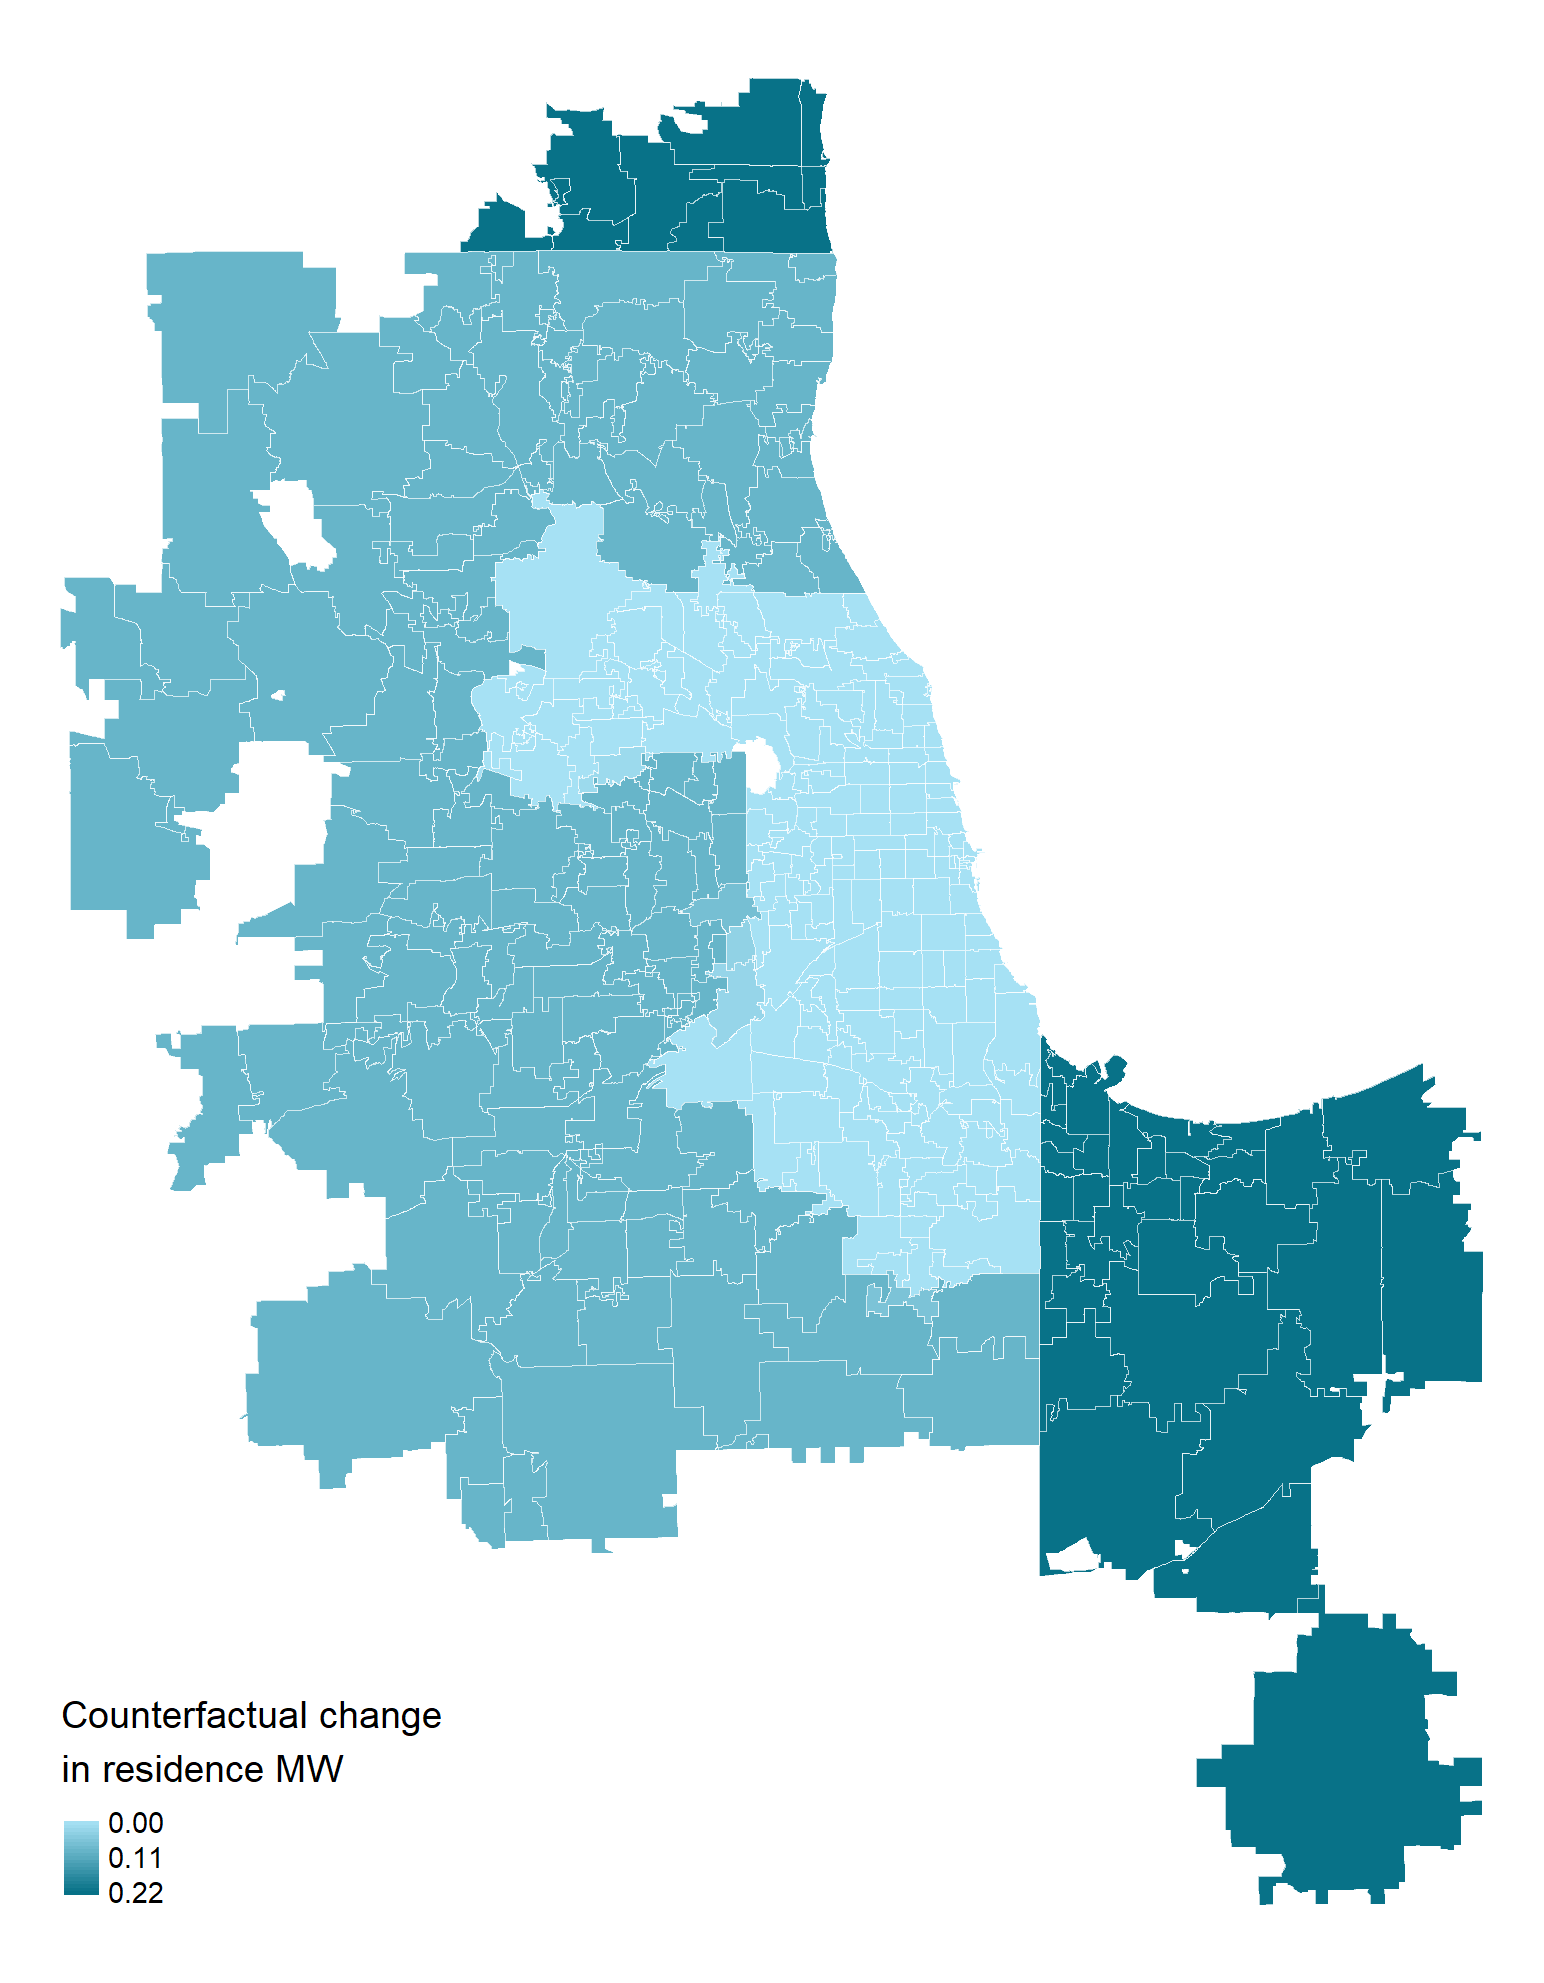
\includegraphics[width = 1\textwidth]
            {counterfactuals/output/chicago_d_mw_res.png}
    \end{subfigure}%
    \begin{subfigure}{.49\textwidth}
        \caption{Counterfactual changes in workplace MW}
        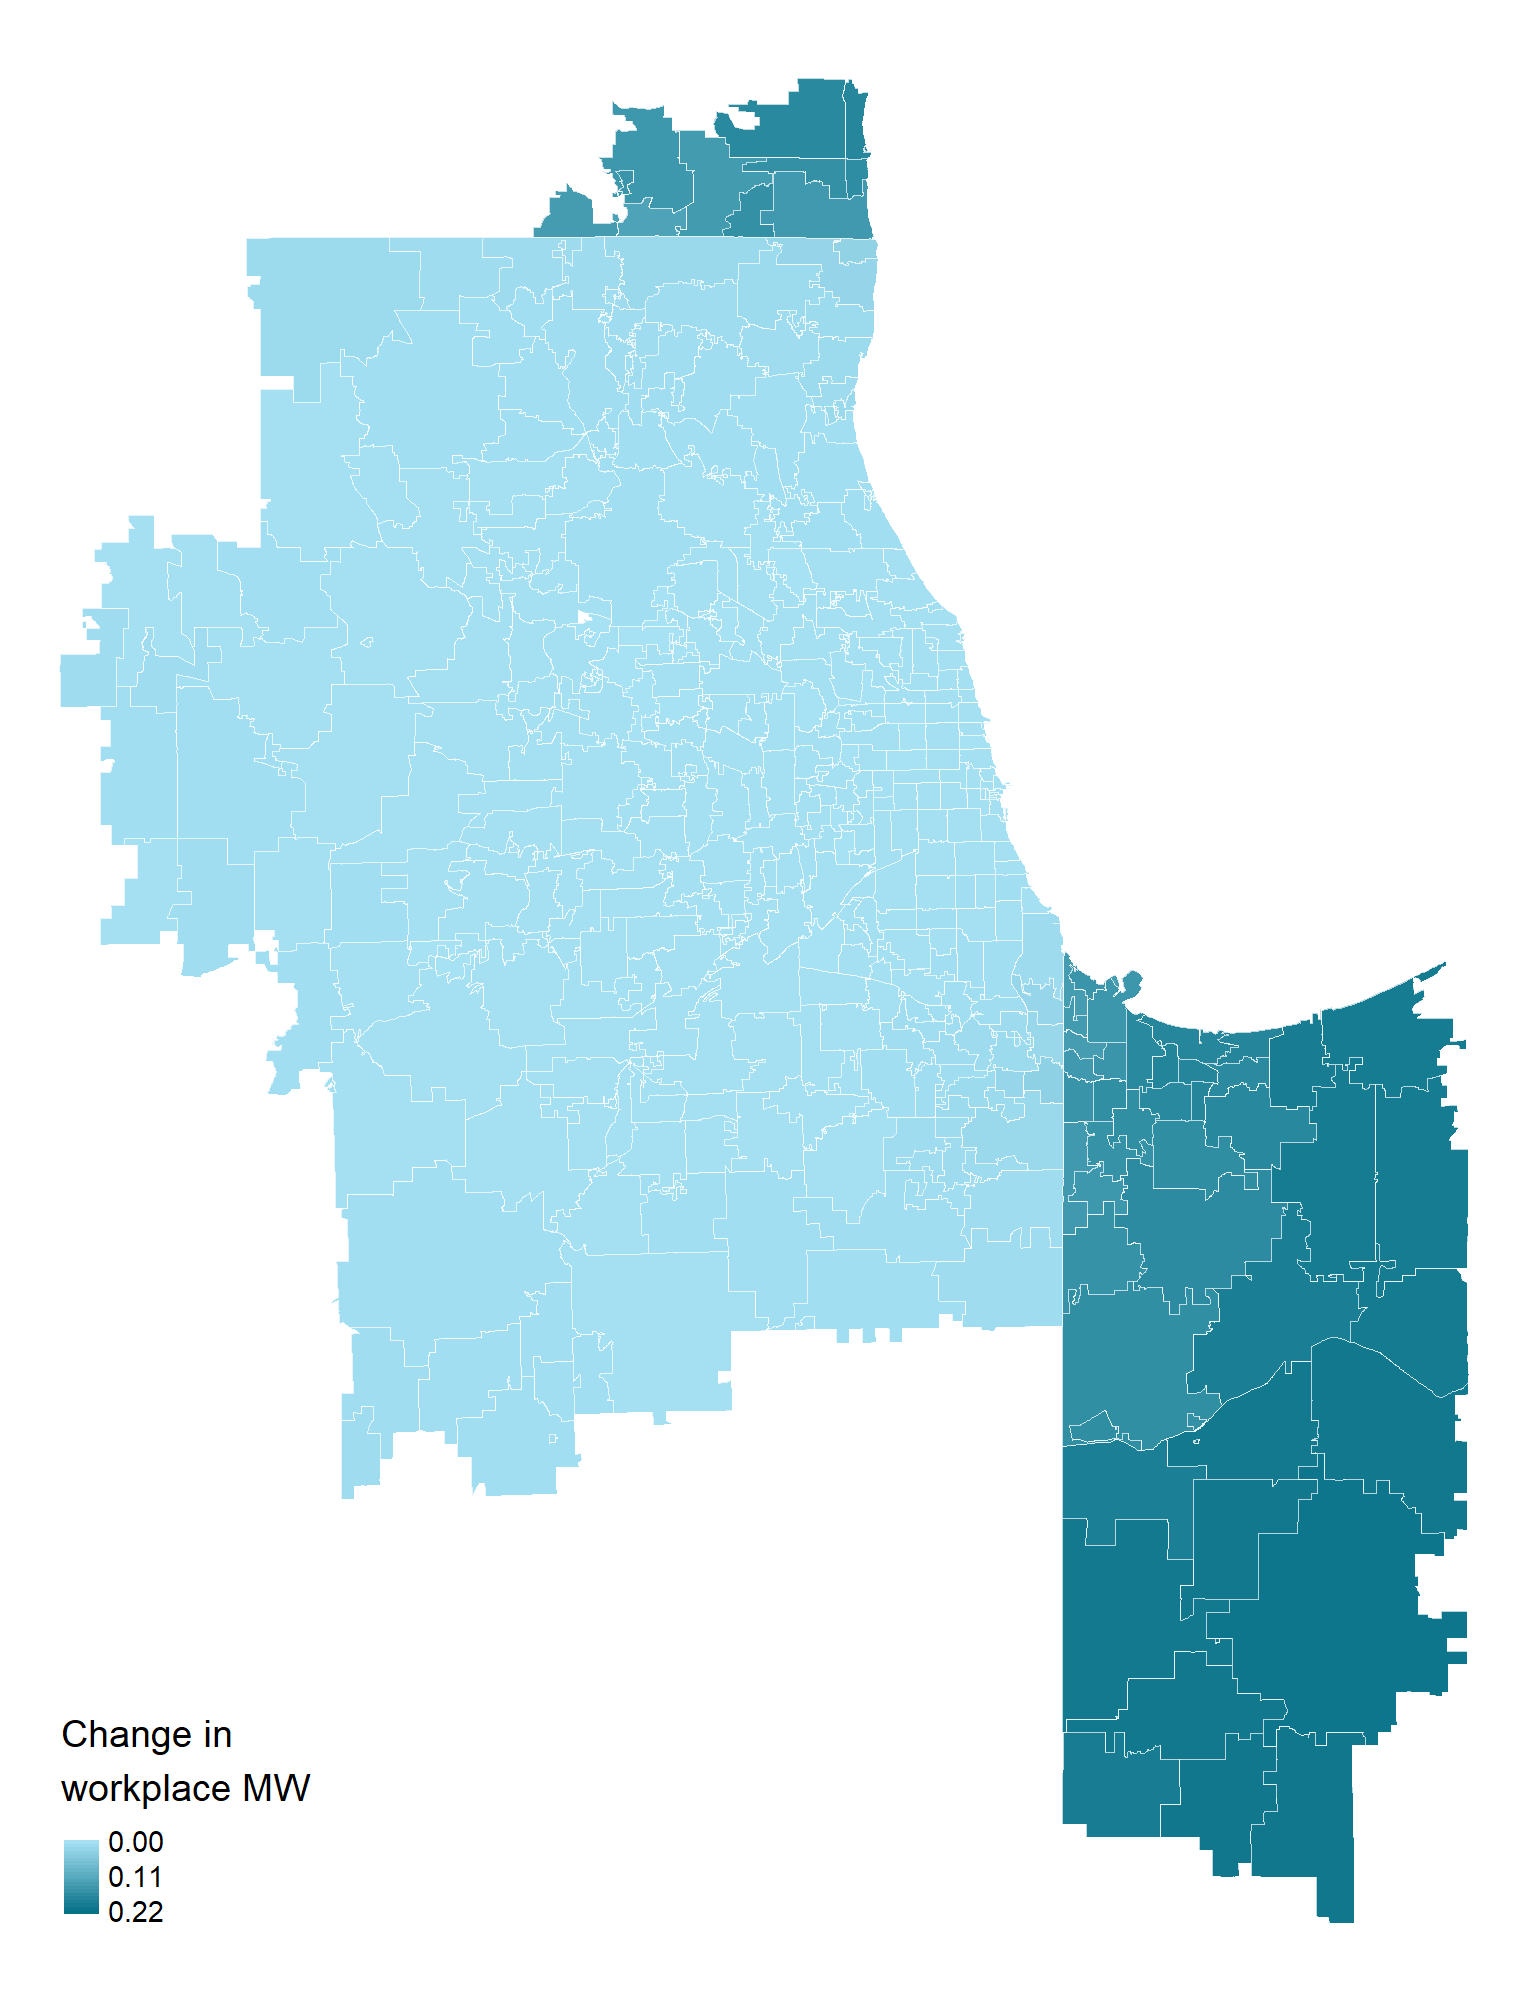
\includegraphics[width = 1\textwidth]
            {counterfactuals/output/chicago_d_mw_wkp.png}
    \end{subfigure}

    \begin{minipage}{.95\textwidth} \footnotesize
        \vspace{3mm}
        Notes:
	Notes: 
    The unit of observation is a ZIP code.
    Panel (a) displays counterfactual changes for the rent per square foot in the 
    Zillow SFCC category computed as explained in Section \ref{sec:cf_rents_and_wage_changes}.
    Panels (b) and (c) display counterfactual changes for the residence and the 
    workplace MW measure computed as explained in Section \ref{sec:cf_res_and_wkp_changes}.
    \end{minipage}
\end{figure}
